% !Mode:: "TeX:UTF-8"

\chapter{}
\textbf{
Given an array $A=<5,13,2,25,37,17,20,8,24,9,7>$, please show:
\begin{enumerate}
  \item $A$ after the BuildHeap(A) process;
  \item $A$ right after heap\_size(A) turns into 8;
  \item $A$ right after heap\_size(A) turns into 3.
\end{enumerate}
}
\hspace*{\fill} \\

1. After the BuildHeap($A$) process, the tree is showed in figure~\ref{A tree_1},and array $A=<37,25,20,24,13,17,2,8,5,9,7>$
\begin{figure}[!htbp]
  \centering
  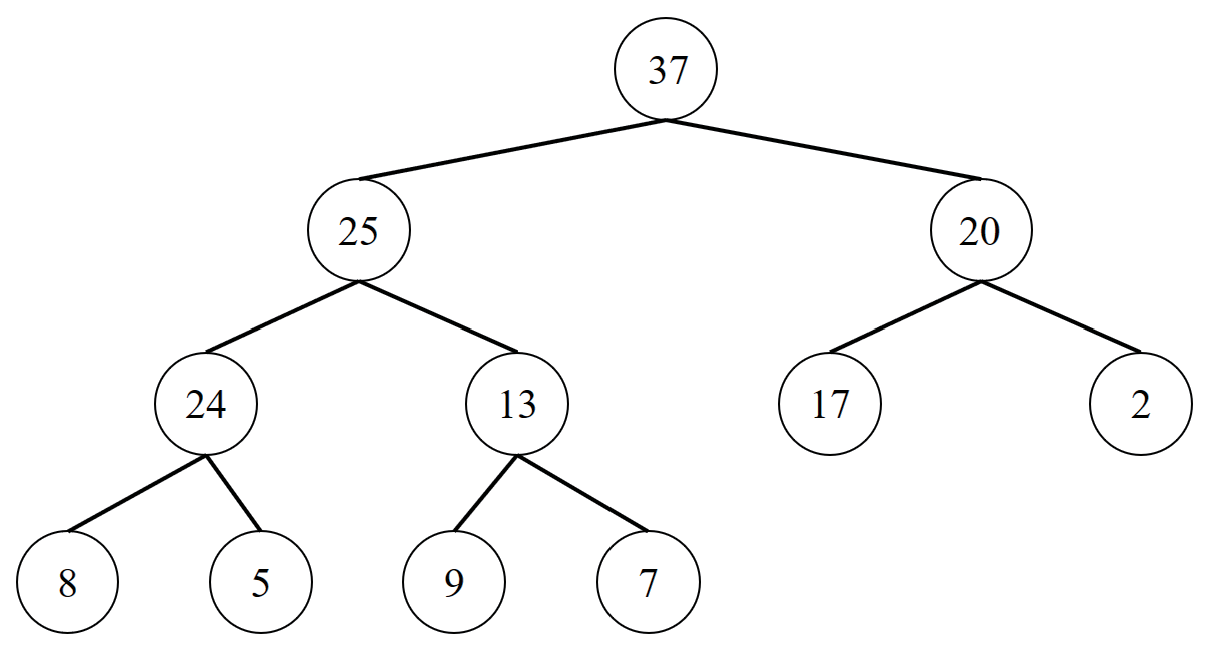
\includegraphics[width=0.5\textwidth]{figures/1.eps}\\
  \caption{After the BuildHeap(A) process}\label{A tree_1}
\end{figure}

2. After heap\_size(A) turns into 8, the tree is showed in figure~\ref{A_tree_2}, and array $A=<37,25,20,8,13,17,2,5>$
\begin{figure}[!htbp]
  \centering
  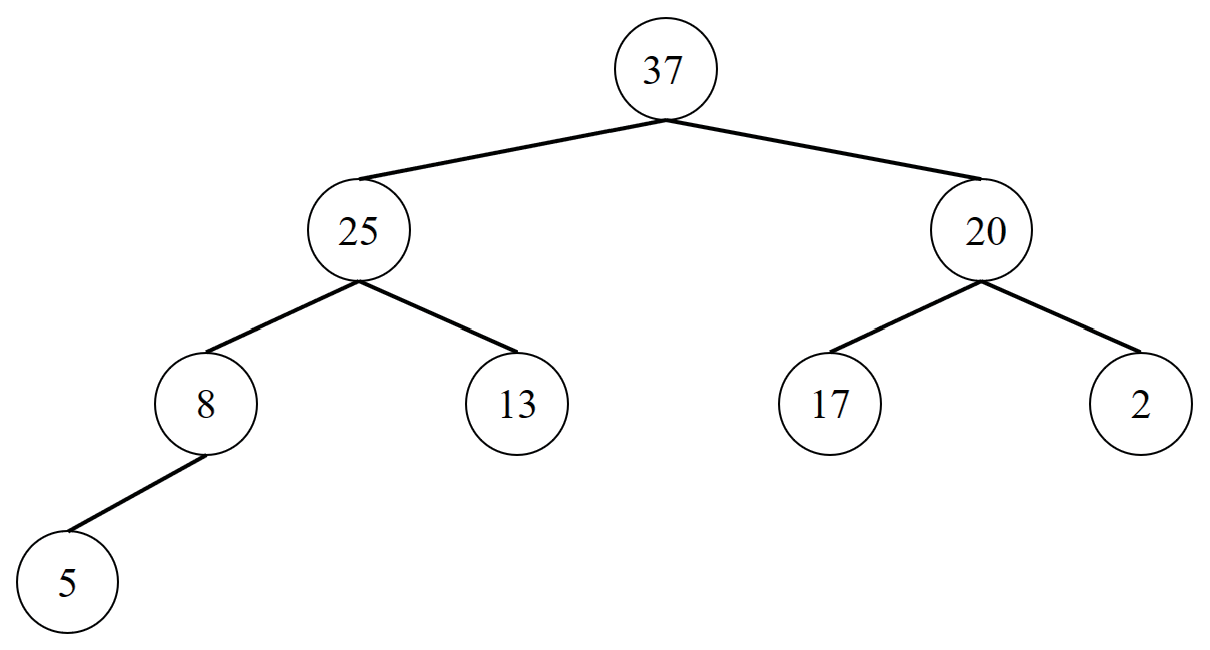
\includegraphics[width=0.5\textwidth]{figures/2.eps}\\
  \caption{after heap\_size(A) turns into 8}\label{A_tree_2}
\end{figure}

3. After heap\_size(A) turns into 3, the tree is showed in figure~\ref{A_tree_3}, and array $A=<13,5,2>$
\begin{figure}[!htbp]
  \centering
  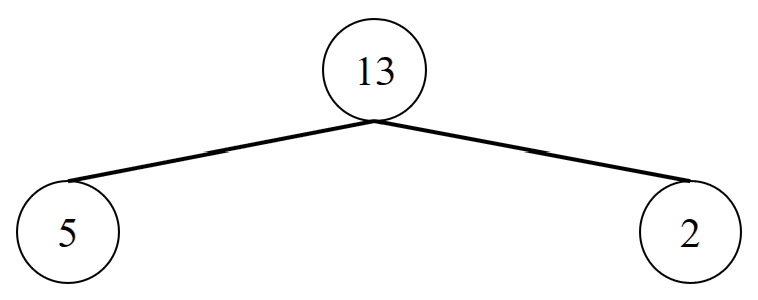
\includegraphics[width=0.5\textwidth]{figures/3.eps}\\
  \caption{after heap\_size(A) turns into 3}\label{A_tree_3}
\end{figure}